\textbf{Исходный текст:} \\
    !?;,:.-

\textbf{Публичный ключ $(e, n)$:} \\
    (1827821233260228957330462119381, 8606963804773339124904139583897)

\textbf{Приватный ключ $(d, n)$:} \\
    (1618330337596630383004261807997, 8606963804773339124904139583897)

\textbf{Зашифрованный текст:} \\
    7682999861805463840962051524493 4403838174454233083555965378737
    1909354241146547364672395621626 6858093156978570257166638594841
    5048676731057660471922055344624 1308786662182323412950422448348
    8590765347481596817223057719572 

Результаты работы программы представлены на рисунках~\ref{ris:encode-test-4}-\ref{ris:decode-test-4}.

\vspace{\baselineskip}
\begin{figure}[H]
\center{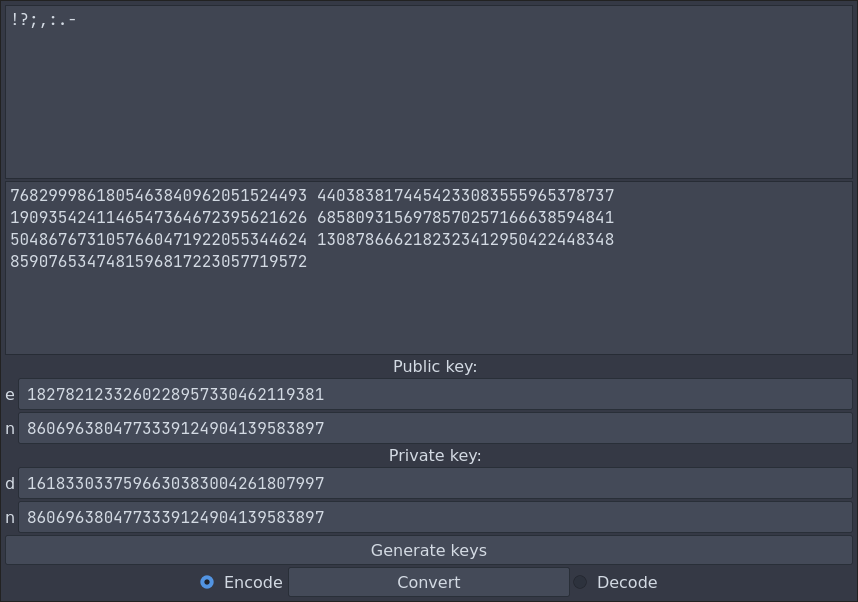
\includegraphics[width=0.8\linewidth]{figures/encode-test-4}}
    \caption{Шифрование}
\label{ris:encode-test-4}
\end{figure}

\vspace{\baselineskip}
\begin{figure}[H]
\center{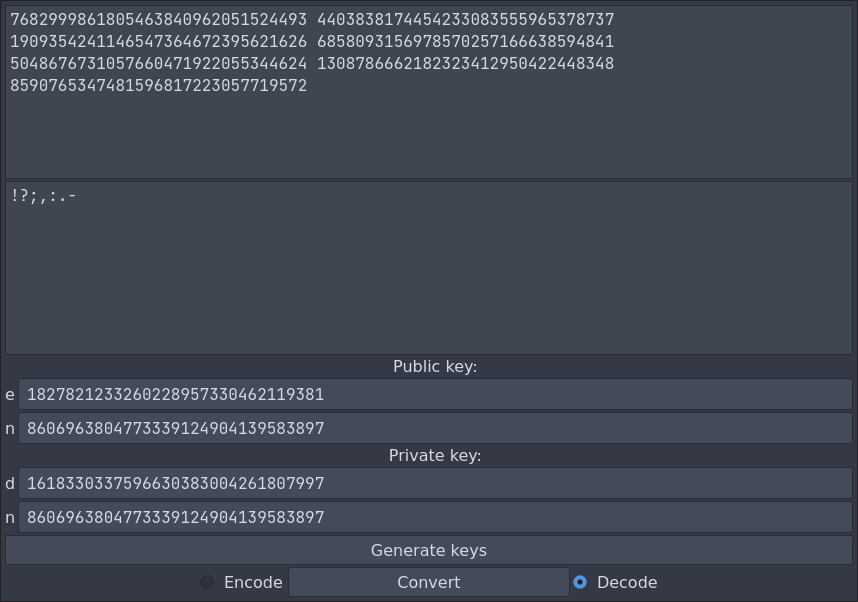
\includegraphics[width=0.8\linewidth]{figures/decode-test-4}}
    \caption{Расшифрование}
\label{ris:decode-test-4}
\end{figure}
